\documentclass{report}
\usepackage{listings}
\usepackage{amsthm}
\usepackage{amsmath}
\usepackage{tcolorbox}
\usepackage{calligra}
\usepackage{siunitx}
\usepackage{url}
\usepackage{float}
\usepackage[labelformat=empty]{caption}

% Create a custom definition environment
\newenvironment{defbox}[1]{%
  \tcolorbox[
    colback=black!5,
    colframe=darkgray,
    title=#1
  ]
}{%
  \endtcolorbox
}


\theoremstyle{definition}

\lstset{
    basicstyle=\ttfamily\small, % Choose the font style and size
    numbers=left,              % Line numbers position
    numberstyle=\tiny,         % Line numbers style
    breaklines=true,           % Automatic line breaking
    frame=single,              % Add a frame around the code
    tabsize=2,                 % Tab size reduced to 2
    showspaces=false,          % Don't show spaces
    showstringspaces=false,    % Don't show spaces in strings
    % Removed all color/syntax highlighting styles
}

% Save the original definitions before redefining them
\let\oldsection\section
\let\oldsubsection\subsection
\let\oldsubsubsection\subsubsection
\let\oldparagraph\paragraph
\let\oldsubparagraph\subparagraph

% Redefine each command to use its starred version
\renewcommand{\section}{\oldsection*}
\renewcommand{\subsection}{\oldsubsection*}
\renewcommand{\subsubsection}{\oldsubsubsection*}
\renewcommand{\paragraph}{\oldparagraph*}
\renewcommand{\subparagraph}{\oldsubparagraph*}

\usepackage{tikz}
\usetikzlibrary{positioning, shapes, arrows, fit, calc}

\usepackage{graphicx}
\usepackage{parskip}

\graphicspath{{images/}}

\begin{document}

\chapter{Proximity Service}

In this chapter we design a proximity service.

\begin{itemize}
\item 
A proximity service is used to discover nearby places such as restaurants, hotels, theaters, museums, etc., and is a core component that powers features like finding the best restaurants nearby on Yelp or finding k-nearest gas stations on Google Maps.
\item
Figure 1.1. shows the user interface via which you can search for nearby restaurans on Yelp [1]
\item
Note the map tiles used in this book are from Stamen Design [2] anbd data are from OpenStreetMap [3]
\end{itemize}

\begin{figure}[H]
  \begin{center}
    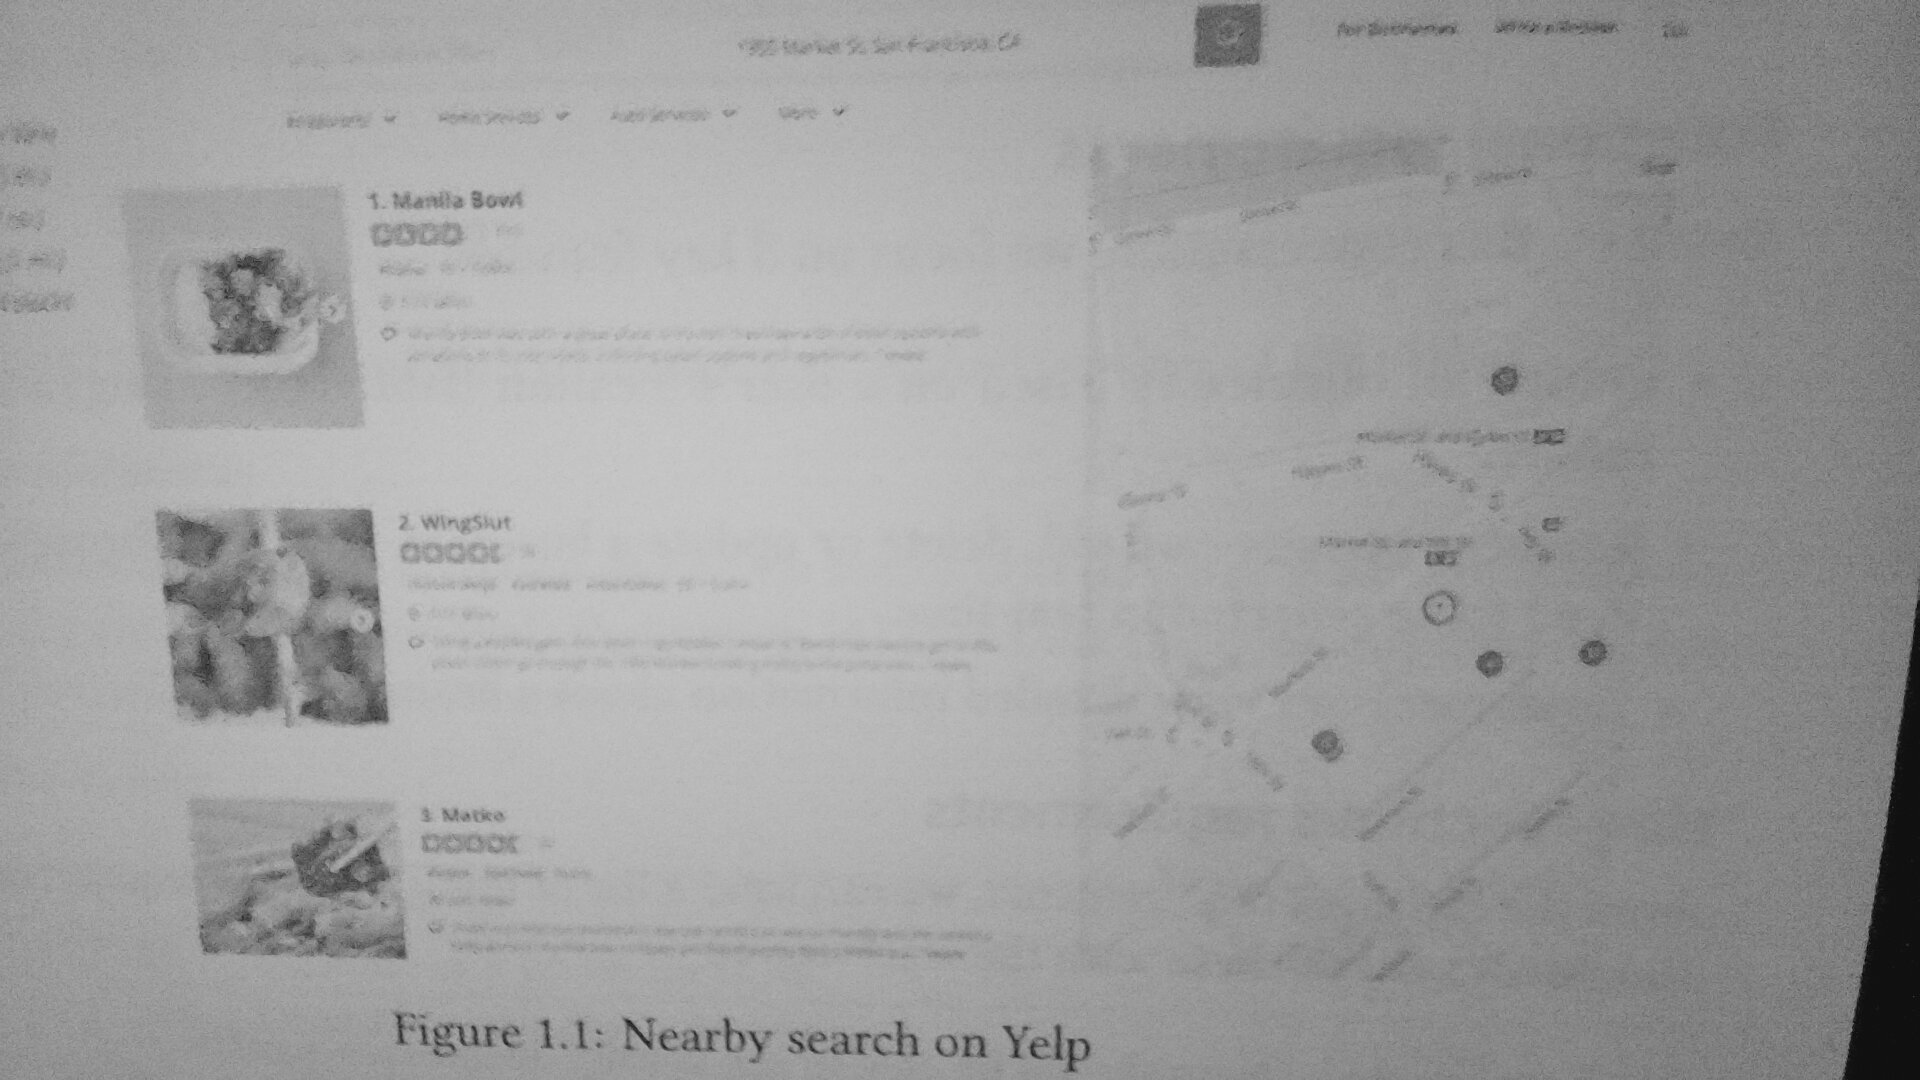
\includegraphics[width=0.8\linewidth]{nearby_search_on_yelp.jpg}
    \caption{Nearby search on yelp}
  \end{center}
\end{figure}

\subsection{Step 1 - Understand the Problem and Establish Design Scope}

Yelp supports many features and it is not feasible to design all of them in an interview seesion, so it's important to narrow down the scope by asking questions

The interactions between the candidate and interviewer could look like this: 

\begin{itemize}
\item 
Candidate: Can a user specify the search radius? If there are not enough businesses within the search raidus, does the system expand the search?
\item
Interviewer: That's a great question. Let's assume we only care about businesses within a specified radius. If time allows, we can then discuss how to expand the search if there are not enough binesses within the radius
\item
Candidate: Can a user change the search radius on the UI?
\item
Interviewer: Yes, we have the following options: 0.5km (0.31 mile), 1km (0.62 mile), 2km (1.24 mile), 5km (3.1 mile), and 20 km (12.42 mile)
\item
Candidate: How does business information get added, deleted, or updated? Do we need to reflect these operations in real-time?
\item
Interviewer: Business owners can add, delete or update a business. Assume we have a business agreement upgfront that newly added/updated businesses will be effective the next day.
\item
Candidate: A user might be moving while using the app/website, so the search results could be slightly different after a while. Do we need to refresh the page to keep the results up to date?
\item
Interviewer: Let's assume a user's moving speed is slow and we don't need to constantly refresh the page
\end{itemize} 

\subsection{Functional requirements}

Based on this conversation, we focus on 3 key features:

\begin{itemize}
\item 
Return all businesses based on a user's location (latitidue and longitude pair) and radius
\item
Business owners can add, delete, or update a business but this information doesn't need to be reflected in real time
\item
Customers can view detailed information about a business
\end{itemize}


\end{document}

